\documentclass[fr]{../../../../../../eplexam}
\usepackage{../../../../../../eplcommon}
\usepackage{../../../../../../eplunits}

\hypertitle{Automatique linéaire - INMA1510}{6}{INMA}{1510}{2018}{Septembre}{Majeure}
{Luis Tascon Gutierrez}
{Denis Dochain}

\section{}

Vélo

Idem question $4$ de Juin $2015$ mais avec plus de paramètres\dots La formulation exacte de la question n'a pas été notée.

Il n'a demandé que de trouver la fonction de transfert et les conditions d'équilibre mais il y avait plus de conditions qu'en $2015$.

\nosolution

\newpage
\section{}
La dynamique d'un circuit composé d'une diode tunnel peut être représentée par:
\begin{gather*}
\begin{aligned}
\dot{x}_1 &= x_2 -h(x_1)\\
\dot{x}_2 &= -x_1 -ux_2 + E
\end{aligned}
\end{gather*}

La variable $x_1$ représente la tension aux bornes de la capacité du circuit. $x_2$ est le courant passant dans l'inductance du circuit. $E$ représente la tension externe et $u$ la tension aux bornes de la résistance du circuit.
\begin{equation*}
h(x_1) = 2x_1^3-6x_1^2+5x_1
\end{equation*}
On a également les valeurs de $E = 1,5$ et $u= 0,5$
\begin{enumerate}
	\item Déterminez le(s) point(s) d'équilibre du circuit.\footnote{Un graphe de $h(x_1)$ était disponible pour nous aider.}
	\item Pour chaque état d'équilibre, analysez la stabilité.
\end{enumerate}

\nosolution

\newpage
\section{}

Soit la fonction de transfert $$G(s) = \dfrac{0.1}{s(s^2+0.02s+0.1)}$$
avec les graphes suivants:

\begin{figure}[!h]
	\centering
	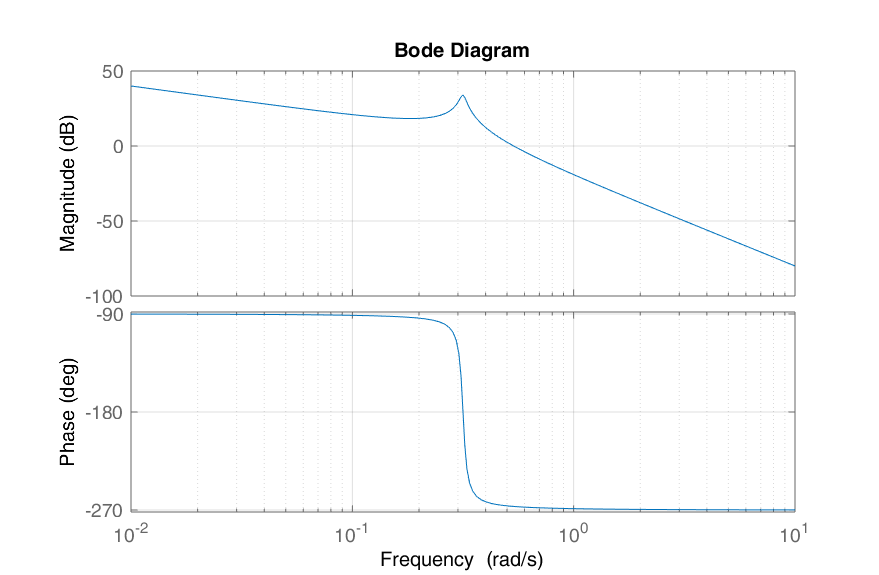
\includegraphics[scale=0.5]{bodeplot.png}
	\caption{Pm = at and Gm = at }
\end{figure}

Trouvez le paramètre $k0$ (prémultiplicateur du compensateur) et les paramètres du compensateur à avance de phase pour qu'on ait dans le système en boucle fermée:

$\Phi_M = \ang{85}$ à la fréquence $w = 0.01$ rad/sec.

\nosolution


\newpage
\section{}
On a la fonction de transfert $G(s) = \dfrac{5 e^{-2 s}}{0.25 s + 1} $.

On souhaite n'avoir qu'un seul pôle en $-5$.
\begin{enumerate}
	\item Quel contrôleur $C(s)$ faut-il employer? À quoi faut-il faire attention?
	\item En utilisant la même forme de compensateur qu'au point $1$, synthétiser une loi de commande qui permette d'éliminer les effets négatifs sur le comportement en boucle fermée. Comment se nomme cette loi de commande? Quelles précautions devez-vous prendre?
	\item Analyser la stabilité en boucle fermée pour les points $1$ et $2$. Quelles sont vos conclusions?
	\item Pour la deuxième configuration, vous avez fait la synthèse en pensant que le retard était $0.4$ (alors que sa vraie valeur est bien $2$). Analysez la stabilité du système en boucle fermée dans ce cas de figure.
\end{enumerate}

Si, à un moment donné de votre démarche, vous devez approximer le retard, utilisez l'approximation de Taylor. 

Justifiez vos réponses.\footnote{Question identique en juin $2017$ pour les majeurs à part pour le retard approximé au point $4$ et quelques formulations légèrement différentes.}
\begin{solution}
	
	\begin{enumerate}
		\item 
		On veut $$Tr(s)=\frac{e^{-2s}}{1+0.2s}$$ 
		Donc $C(s)=\frac{1}{44}\left(1+\frac{4}{s}\right)$.
		
		\item 
		Dans ce paragraphe $G(s)$ est la fonction qui décrit le système sans considérer le retard $e^{-\theta s}$.
		Une structure de contrôle qui annule les effets du retard n'existe pas. Mais on peut empêcher que ce retard sur $G(s)$ ne déstabilise le système grâce à un prédicteur de Smith. Le prédicteur de Smith permet de transférer le retard de $G(s)$ vers la fonction de transfert $Tr(s)$. Cette structure de contrôle est composée d'un compensateur et un boucle de rétroaction négative non-unitaire de la forme $G(s)(1-e^{-\theta s})$. Le paramètre $\theta$ (le retard) doit être connu a priori sinon le prédicteur de Smith n'est pas optimal. Voici la fonction de transfert d'un prédicteur de Smith:
		$$ C_{Smith}(s) = \dfrac{C(s)}{1+(1-e^{-\theta s})C(s)G(s)}$$
		$$Tr(s) = \dfrac{C_{Smith}(s)G(s)e^{-\theta s}}{1+C_{Smith}(s)G(s)e^{-\theta s}} = \dfrac{C(s)G(s)}{1+C(s)G(s)}e^{-\theta s}$$
		
		Donc $C(s)=\frac{1}{4}\left(1+\frac{4}{s}\right)$
		
		\item Les 2 systèmes sont stables, tant que l'approximation de Taylor reste valable.
		
		\item Cette sous-question n'a pas encore de réponse.
	\end{enumerate}
	
\end{solution}

\newpage
\section{}
Quel contrôleur faut-il employer pour avoir une erreur statique nulle avec une consigne $r(t) = \gamma \sin{b t}$? Démontrer.\footnote{Question identique en juin $2017$ pour les majeurs.}

\begin{solution}
	
	Imaginons une boucle de rétroaction négative avec un compensateur $C(s)$ sans système $G(s)$ à contrôler, la consigne est noté $r(t)$ et la sortie $y(t)$. $C_o(s)$ est le numérateur du compensateur. Son degré est toujours inférieur à celui du dénominateur.
	
	Formule générale:
	$$ C(s) = \dfrac{1}{s^{q+1}} \prod\limits_{k=1}^p \left(\dfrac{1}{s^2+w_k^2}\right)C_o(s)$$
	
	L'erreur est notée $e(t)$. 
	$$y(t)=\gamma\,|Tr(jb)|\sin\left[b\,t+\arg(Tr(jb))\right]$$
	
	$$e_h = 0 \qquad \Longleftrightarrow \qquad Tr(jb)=1$$
	
	$$\frac{C(jb)G(jb)}{1+C(jb)G(jb)}=\frac{C_0(jb)G(jb)}{(s^2+b^2)+C_0(jb)G(jb)}=1$$
	Donc $C(s) = \dfrac{C_o(s)}{(s^2+b^2)}$ annule l'erreur statique.
	
\end{solution}

\newpage
\section{}
On a le système suivant :
\begin{equation*}
\left \{
\begin{array}{l @{} l}
\dot{x} = A x + B u \\
y = C x \\
\end{array}
\right.
\hspace{0.5cm}
A = 
\begin{pmatrix} 
0 & 2 \\
1 & 4
\end{pmatrix}
\hspace{0.3cm}
B = 
\begin{pmatrix} 
0 \\
1 
\end{pmatrix}
\hspace{0.3cm}
C = 
\begin{pmatrix} 
1 & 0
\end{pmatrix}
\end{equation*}
Considérer une commande quadratique linéaire.

\begin{itemize}
	\item Trouvez les coefficients de la matrice P qui est solution de l'équation de Riccati et le gain K associé si les matrices $Q_x$ et $Q_u$ sont toutes deux des matrices unités.
	\item Quelle est la dynamique en boucle fermée du système? Quelles sont vos conclusions?
\end{itemize}

\begin{solution}
\begin{enumerate}
	\item La matrice $P$ qui est symétrique et définie positive est solution de l'équation de Riccati:
	$$M = A^TP+PA-PBQ_u^{-1}B^TP+Q_x = 0$$
	On a donc:
	$$A^TP = \begin{pmatrix}0 & 1\\ 2 & 4 \end{pmatrix}\begin{pmatrix} p_1 & p_2 \\ p_2 & p_3 \end{pmatrix} = \begin{pmatrix} p_2 & p_3 \\ 2p_1+4p_2 & 2p_2+4p_3\end{pmatrix}$$
	$$PA = \begin{pmatrix} p_1 & p_2 \\ p_2 & p_3 \end{pmatrix}\begin{pmatrix}0 & 2\\ 1 & 4 \end{pmatrix} = \begin{pmatrix} p_2 & 2p_1+4p_2 \\ p_3 & 2p_2+4p_3\end{pmatrix}$$
	Vu que $Q_u^{-1}$ est une matrice unité, on peut l'ignorer dans la multiplication matricielle.
	$$PBB^TP = \begin{pmatrix} p_1 & p_2 \\ p_2 & p_3 \end{pmatrix} \begin{pmatrix}0 & 0 \\ 0 & 1\end{pmatrix} \begin{pmatrix} p_1 & p_2 \\ p_2 & p_3 \end{pmatrix} = \begin{pmatrix}p_2^2 & p_2p_3\\ p_2p_3 & p_3^2\end{pmatrix}$$
	On a donc:
	$$M = \begin{pmatrix} p_2 & p_3 \\ 2p_1+4p_2 & 2p_2+4p_3\end{pmatrix} + \begin{pmatrix} p_2 & 2p_1+4p_2 \\ p_3 & 2p_2+4p_3\end{pmatrix} - \begin{pmatrix}p_2^2 & p_2p_3\\ p_2p_3 & p_3^2\end{pmatrix} + \begin{pmatrix}1 & 0 \\ 0 & 1\end{pmatrix} = \begin{pmatrix}0 & 0\\0 & 0\end{pmatrix}$$
	Qui nous donne 3 équations à 3 inconnues (il y a 2 équations identiques car P est symétrique).
	$$\begin{cases} -p_2^2+2p_2+1 = 0\\ -p_2p_3+2p_1+4p_2+p3+1 = 0 \\ -p_3^2+4p_2+8p_3+1 = 0 \end{cases}  $$
	Ce qui nous donne les possibilités suivantes (en valeurs approximées) avec $\lambda_1$ et $\lambda_2$ les valeurs propres de la matrice $P$:
	$$\begin{array}{c|c|c|c|c}
	p_1 & p_2 & p_3 & \lambda_1 & \lambda_2\\
	\hline
	1.1510 & 1.4142 & 9.1630 & 0.4798 & 9.8342\\	
	-6.1506 & 1.4142 & -1.1630 & -0.1859 & -7.1277\\	
	-5.2697	& -0.4142 & 7.9170 & -5.6978 & 8.3451\\	
	0.2697 & -0.4142 & 0.0830 & -0.2482 & 0.6009\\	
	\end{array} $$
	Comme on peut l'observer dans le tableau, il n'y a qu'une seule solution qui obtient une matrice définie positive. On est donc sûr et certains d'avoir pour matrice $P$:
	$$P = \begin{pmatrix}1.1510 & 1.4142 \\ 1.4142 & 9.1630\end{pmatrix}$$
	
	On peut maintenant calculer le gain $K$ associé grâce à la formule: $K = -Q_u^{-1}B^TP$. Vu que $Q_u$ est la matrice identité, on peut l'ignorer.
	$$K = \begin{pmatrix}k_1 & k_2\end{pmatrix} = \begin{pmatrix}0 & 1\end{pmatrix}\begin{pmatrix}p_1 & p_2 \\ p_2 & p_3\end{pmatrix}$$
	On a donc le gain $K$ qui vaut:
	$$K = \begin{pmatrix}p_2 & p_3\end{pmatrix} = \begin{pmatrix}1.4142 & 9.1630 \end{pmatrix}$$
	
	\item Cette sous-question n'a pas encore de solution.
\end{enumerate}
\end{solution}

\end{document}
